\documentclass[11pt]{article}
\usepackage[a4paper,margin=22mm]{geometry}
\usepackage[T1]{fontenc}
\usepackage{lmodern,microtype,amsmath,amssymb,graphicx,caption,booktabs,array,tabularx}
\usepackage[super,sort&compress]{natbib}
\usepackage{hyperref}
\hypersetup{colorlinks=true,urlcolor=blue,citecolor=blue,linkcolor=blue,pdftitle={Choosing scientific visualizations through task-first optimization},pdfauthor={Mohamed Elgendi}}
\setlength{\parskip}{5pt}\setlength{\parindent}{0pt}\emergencystretch=4em
\widowpenalty=10000\clubpenalty=10000
\newcommand{\HardAssociation}{-0.000013 [-0.000301, +0.000271]}
\newcommand{\SoftAssociation}{+0.000660 [+0.000236, +0.001163]}
\newcommand{\GeometryShared}{13}
\newcommand{\GeometryPie}{13}
\newcommand{\GeometryDonut}{13}
\newcommand{\GeometryBar}{10}
\newcommand{\GeometryStack}{1}
\title{Choosing scientific visualizations through task-first optimization}
\author{Mohamed Elgendi\\\small Department of Biomedical Engineering and Biotechnology,\\\small Khalifa University, Abu Dhabi, United Arab Emirates}
\date{}
\begin{document}\maketitle
\begin{abstract}
A chart can receive a high numerical score without improving on a simple alternative. We present a reproducible computational benchmark that asks what information a chart should preserve, measures recovery of that information from rendered pixels, and tests whether choosing a different chart for each dataset improves on a strong task-specific default. Six questions cover group differences, category shares, ordered profiles and association. The empirical benchmark contains 530 task instances derived from nine public resources, with 13 familiar chart families and explicit distributional controls. Choices made at 256 pixels are frozen and tested at 384 pixels with shifted placements. Under the primary image-reading algorithm, case-specific selection shows no consistent advantage over defaults learned without the held-out resource or patient. Newly generated synthetic cases reveal benefits for composition and association, but losses for median and spread estimation. A separately implemented geometry decoder changes composition-chart rankings, demonstrating that performance belongs to the chart--decoder combination. The benchmark separates omitted information, pixel-recovery error and transfer performance, and includes complete inputs, code, case-level results and verification. It supports auditable tests of computational chart selection; human comprehension remains a distinct, untested outcome.
\end{abstract}

\section*{Introduction}
A researcher comparing two groups may want to know whether their typical values differ, whether one group is more variable, or whether their distributions differ in several places. These questions require different information. A chart showing group means cannot, in general, answer a question about spread. A chart preserving the requested information may still be difficult for a particular reader or algorithm to interpret. Chart selection therefore needs both a clear question and a clear test of success.

Visualization research provides established task descriptions, design rules and recommendation systems.\cite{amar2005,brehmer2013,mackinlay1986,draco,vizml} Graphical-perception experiments test how people judge visual quantities.\cite{cleveland1984,heer2010} These approaches address different outcomes: a recommended design, agreement with existing design choices, or a reader's performance. Our question is narrower: how accurately can a specified algorithm recover a requested numerical quantity from an implemented chart? We call this image-reading algorithm a decoder. This computational question permits exact targets and reproducible tests, but it does not supply a model of human understanding.

Machine chart-understanding benchmarks address a related problem. ChartQA evaluates visual and logical question answering, while ChartBench tests complex chart reasoning and numerical reliability.\cite{chartqa,chartbench} The present study varies the chart encoding for the same source data and numerical question, then tests the incremental benefit of selection against a fixed default. Its calibrated decoders do not perform open-ended language reasoning or infer unknown axes. This narrower setting makes the encoding, recovery mechanism and comparison policy separately inspectable.

A further distinction is essential. Finding the lowest error among several charts on one display establishes an in-sample minimum. It does not establish that repeatedly selecting charts is useful. A single well-chosen chart might perform equally well on new displays or new inputs. Large gains against a chart that omits the target information can conceal this possibility. Strong fixed defaults must therefore be central to the evaluation, particularly when a proposed selector is presented as a general aid to scientific communication.

We develop an executable benchmark around three questions: \emph{What answer should the chart preserve? Can that answer be recovered from its pixels? Does selection improve on a strong default after conditions change?} The benchmark covers six numerical tasks and keeps the data, rendering, decoder and loss explicit (Fig.~\ref{fig:workflow}). It combines public biomedical examples with newly generated synthetic stress cases. These data provide varied numerical structures; they are not used to infer disease mechanisms or validate clinical decisions.

The main finding is a limit on adaptive selection: its apparent advantage becomes small or inconsistent when appropriate defaults are included. Additional experiments show where selection helps and how changing the decoder changes the ranking. These findings make the benchmark useful even when no new selector wins. They identify what must be demonstrated before a chart-ranking score can support a broader recommendation.

\section*{Results}
\subsection*{The question defines the quantity to preserve}
The six primary tasks are median difference, interquartile-spread difference, five distributional gaps, category shares, an ordered numerical profile and Pearson correlation (Table~\ref{tab:tasks}). A \emph{task specification} records the input structure, target, eligible chart implementations, display conditions, recovery algorithm and loss. Compatibility is attached to an implementation, not merely to a chart-family name: a heatmap can encode a distributional strip or a joint probability grid, and each needs its own recovery rule.

The empirical evaluation uses 127 two-group comparisons from nine resources for each of the first three tasks, 24 compositions, 72 profiles and 53 associations: 530 task instances in total. These are derived views of existing data, not 530 independent cohorts or participants. Thirteen familiar families are implemented across the tasks. Empirical cumulative distribution functions and explicit quantile markers provide additional controls for the marginal tasks. Every tested configuration is retained in the electronic results, including failures and non-winners. Mean bars remain labeled lossy diagnostic controls; an occasional low error cannot establish that they contain an omitted target.

\begin{table}[ht]\centering\small
\caption{\textbf{Six questions and their recovery targets.} Candidate counts refer to fixed implementations, not tuning searches. Losses are compared within tasks; their scales are not interchangeable.}\label{tab:tasks}
\begin{tabularx}{\linewidth}{p{2.6cm}X p{4.1cm}r}\toprule
Question & Target & Loss & Candidates\\\midrule
Typical-value difference & Difference of medians & Absolute error / pooled SD & 10\\
Spread difference & Difference of interquartile ranges & Absolute error / pooled SD & 10\\
Distributional differences & Gaps at five specified percentiles & Mean absolute error / pooled SD & 10\\
Category shares & Vector of category proportions & Total variation & 4\\
Ordered profile & Twelve successive bin means & Mean absolute error / profile SD & 4\\
Association & Pearson correlation of displayed pairs & Absolute correlation error / 2 & 2\\\bottomrule
\end{tabularx}
\end{table}

For a chart $c$, task $t$ and display condition $e$, the decoder receives the image and public calibration such as axes, geometry and colors. It receives neither the observations nor the numerical target. Four placements are rendered and the recovery losses averaged:
\begin{equation}
 L_{c,t,e}=\frac14\sum_{r=1}^{4}\ell_t\bigl(\widehat T_{c,t,e,r},T_t\bigr),
 \qquad S_{c,t,e}=\frac{100}{1+L_{c,t,e}}.
\end{equation}
The optional score $S$ expresses the same error on a scale with a maximum of 100. It preserves the ordering and ties of $L$ exactly; it is not a percentage of readers who understand the chart. The primary results report losses and paired differences rather than treating the score transformation as a methodological contribution.

\begin{figure}[p]\centering
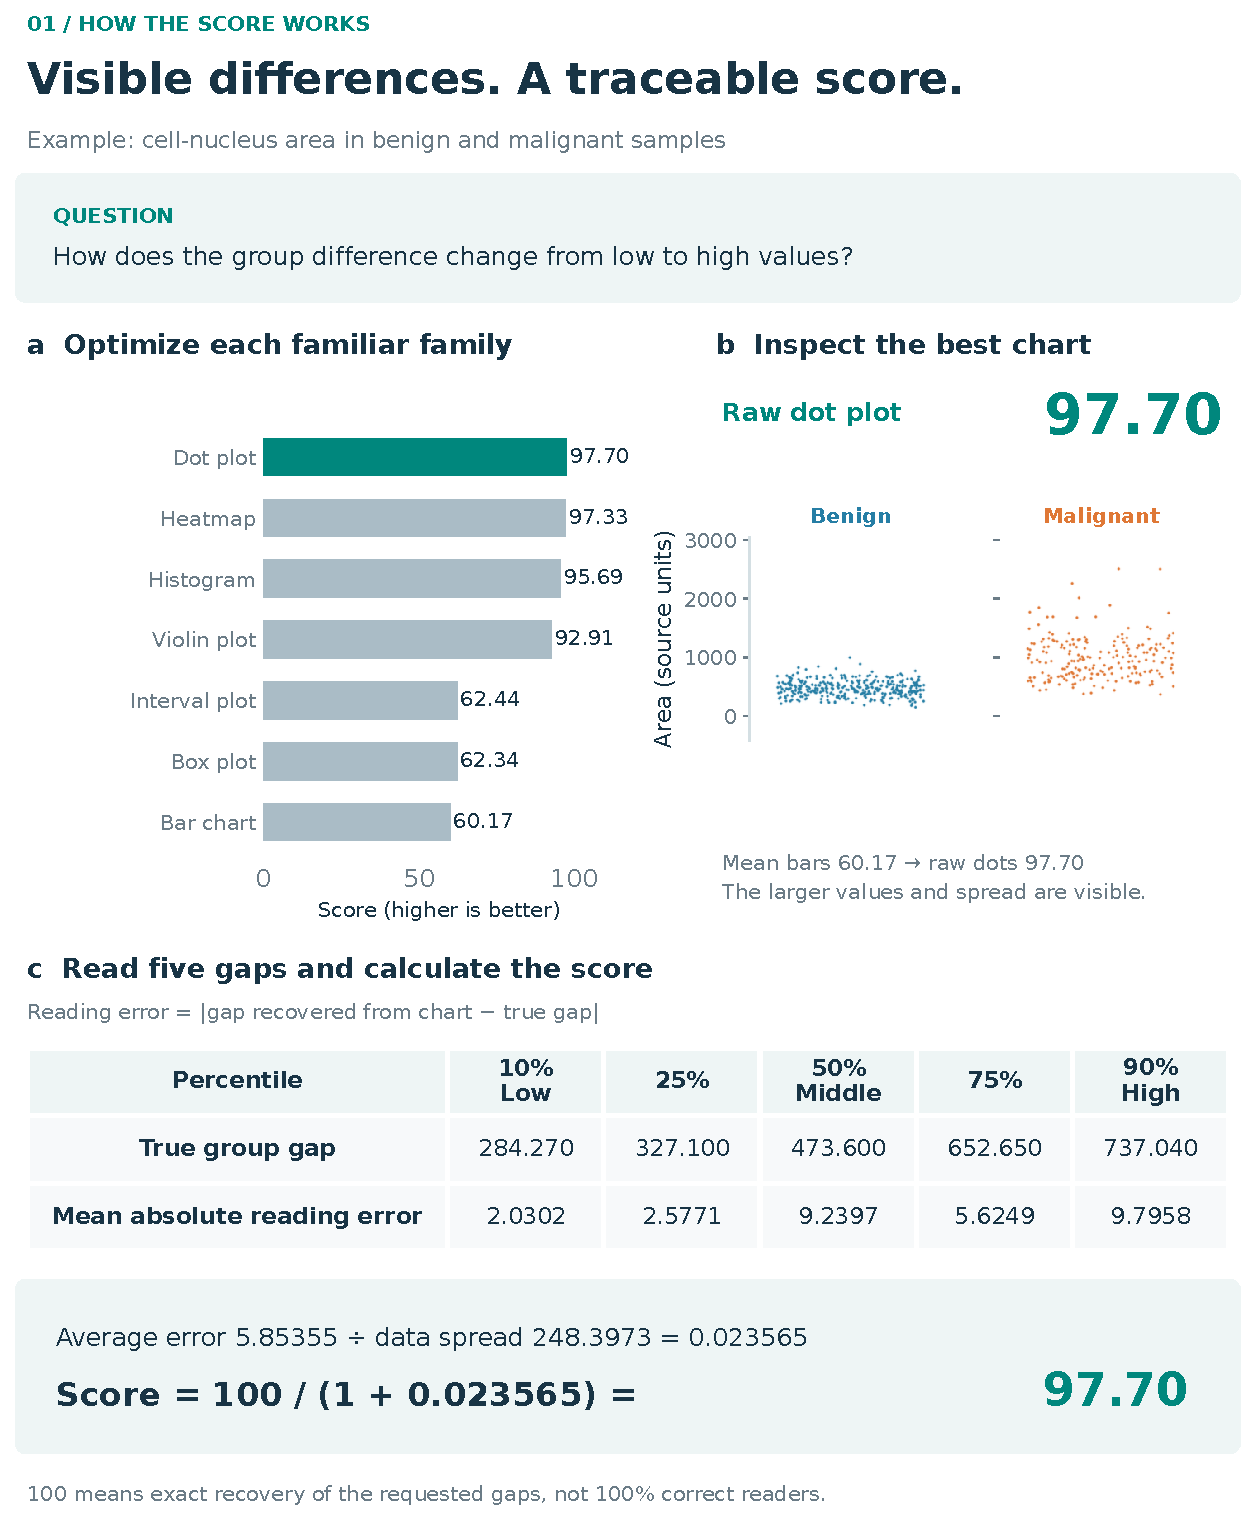
\includegraphics[width=\linewidth,height=.83\textheight,keepaspectratio]{reader_figures/figures/Figure_1_How_scoring_works.pdf}
\caption{\textbf{From a scientific question to an auditable score.} WDBC mean cell-nucleus area compares 357 benign and 212 malignant records. The question asks for five between-group percentile gaps. The display shows the true gaps, recovered errors and score calculation. Dots score 97.70 versus 60.17 for mean bars in the secondary 21-setting familiar-family search. This explains recovery of omitted distributional information; it is not the strong-default comparison. Explicit percentile controls remain in the primary ten-configuration analysis. Scores measure the implemented algorithm's recovery, not human understanding.}\label{fig:workflow}
\end{figure}

\subsection*{Simple examples explain the choice without establishing general benefit}
Figure~\ref{fig:examples} preserves eight concrete, familiar-chart examples: dots, histograms, violins, heatmaps, boxes, pies, lines and scatter plots. Each panel states the question, shows two charts and reports their scores. The seven-family marginal subset uses one fixed setting per family, unlike Figure~\ref{fig:workflow}'s tuning search. These cases were chosen retrospectively to show different computed winners; they are not a representative sample and do not estimate an average benefit.

The box-plot example asks about the difference in interquartile spread of cell-boundary measurements. A box carries quartile information; a mean bar omits it. The pie example asks for observed category shares, where the numerical improvement is only 0.225 score points. The examples teach how the question changes what must be encoded. Whether the chosen chart beats an adequate, fixed alternative requires the separate test below.

\begin{figure}[p]\centering
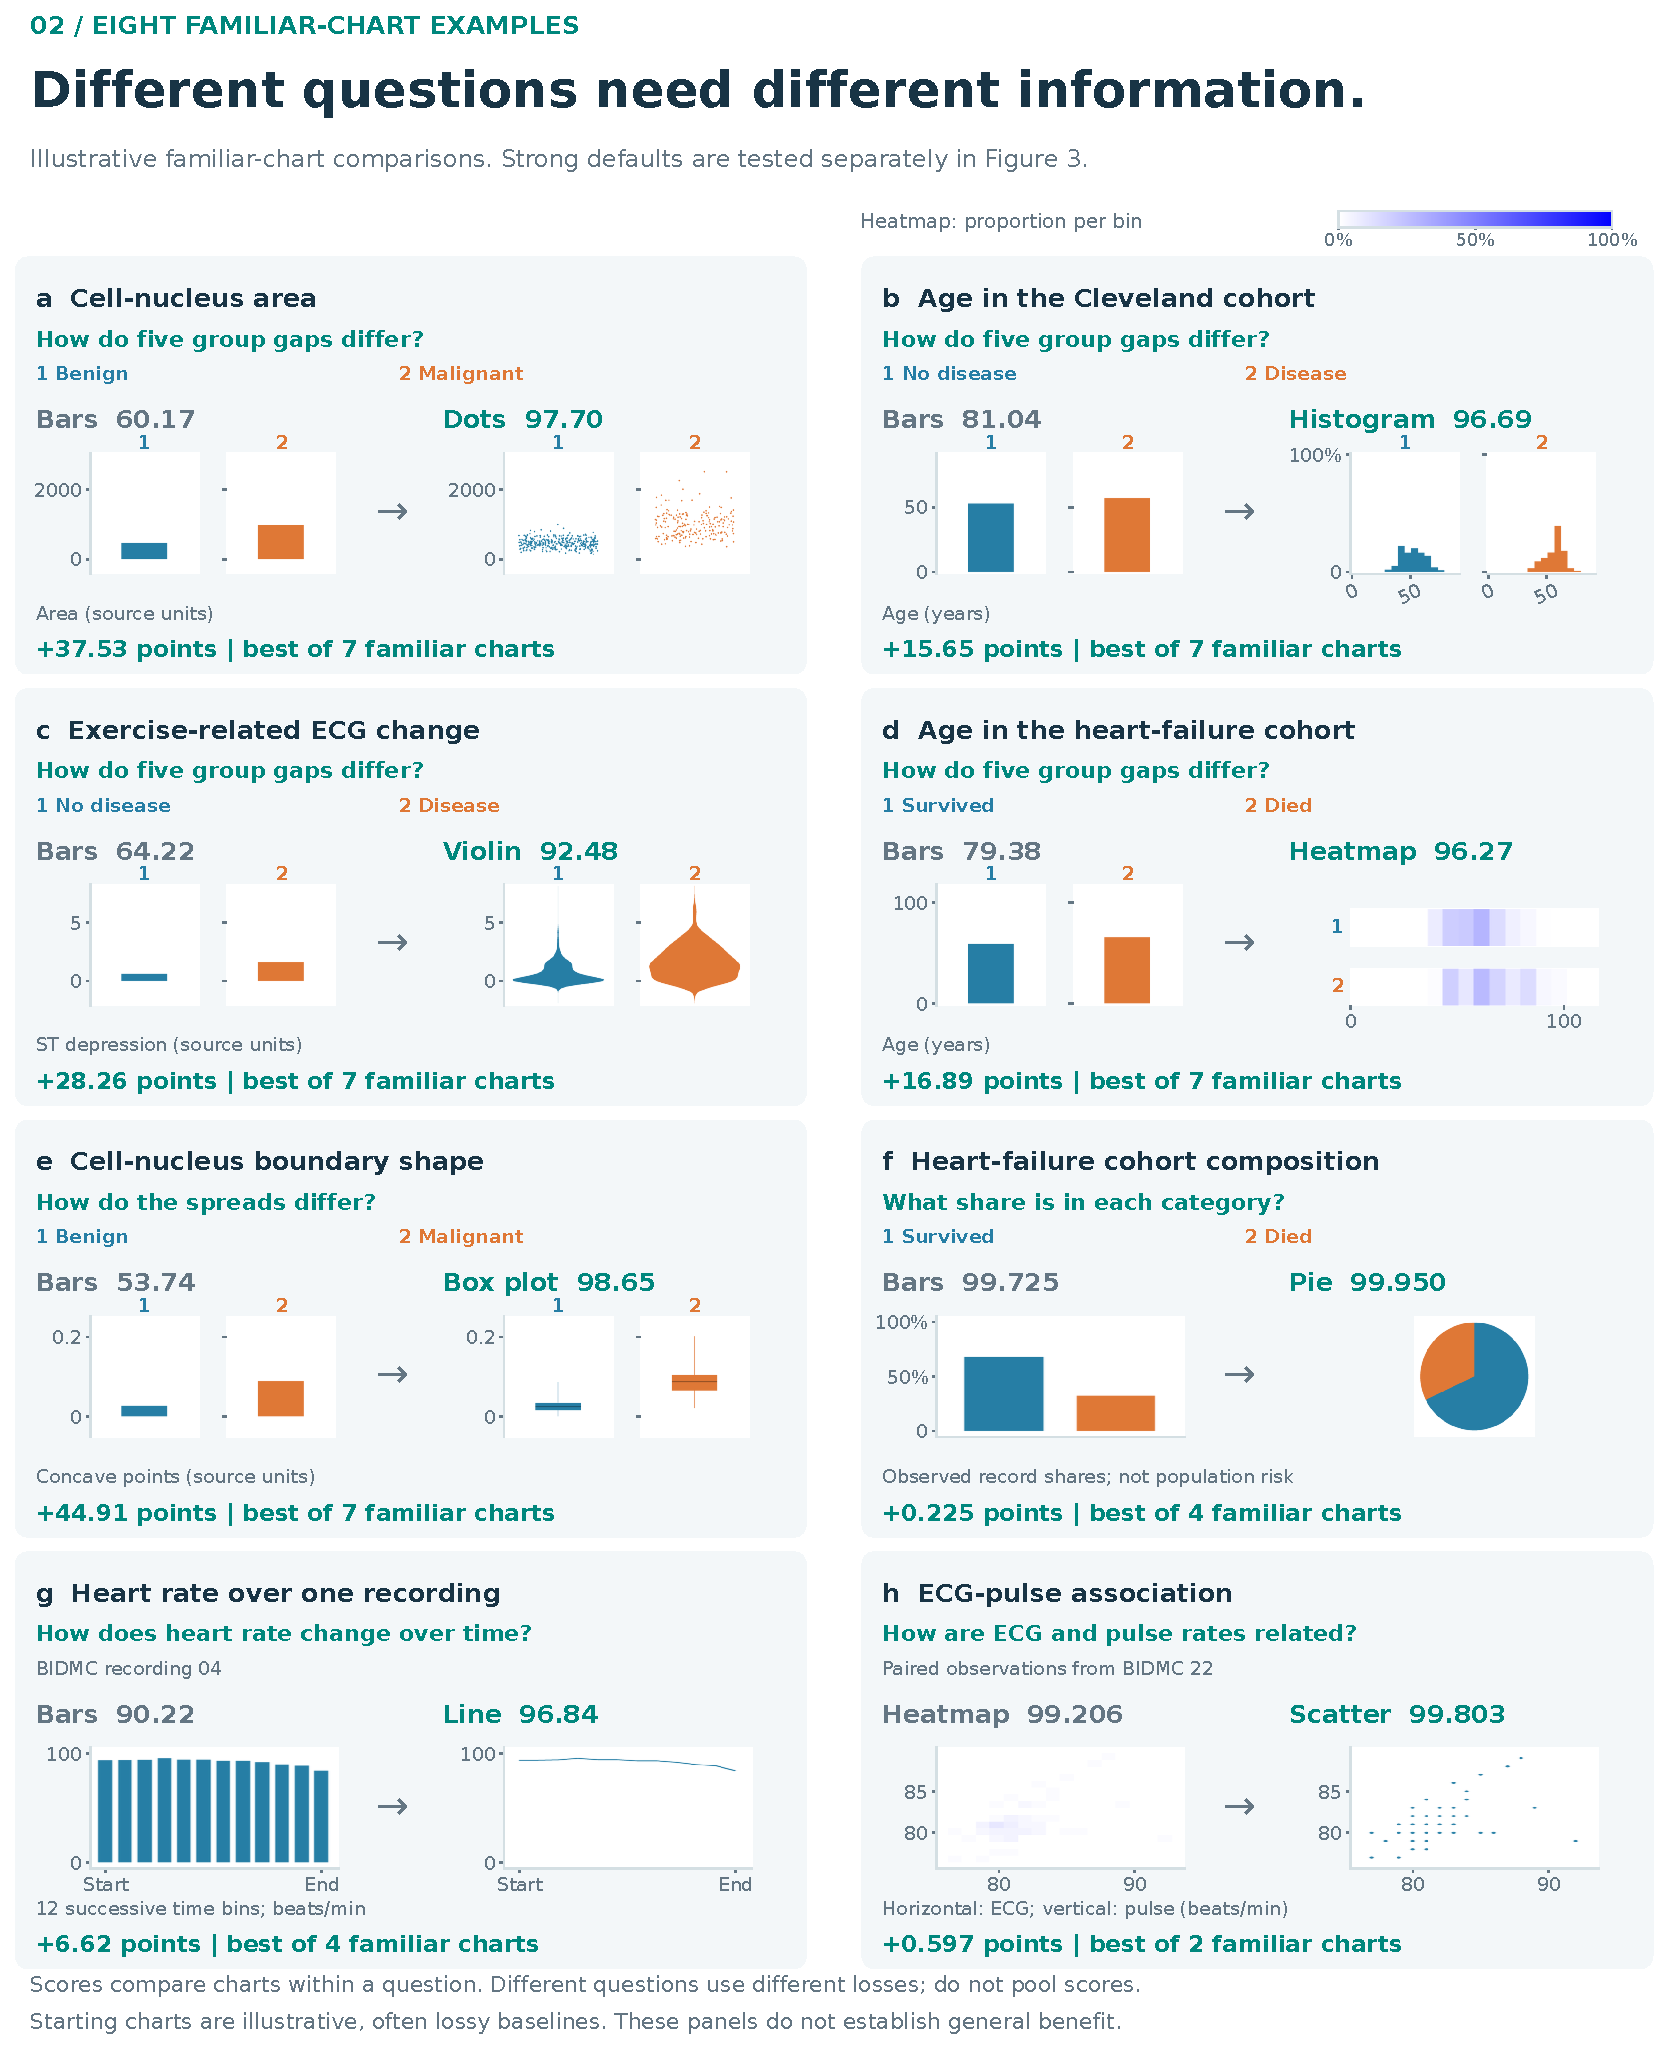
\includegraphics[width=\linewidth,height=.83\textheight,keepaspectratio]{reader_figures/figures/Figure_2_When_optimization_helps.pdf}
\caption{\textbf{Eight familiar examples make the task visible.} Each panel reports a retrospectively selected winner within its implemented familiar-chart subset. Comparisons are within panels only. The starting chart is illustrative and is often a mean bar that omits the requested distributional information. Consequently, the displayed score gaps do not establish benefit over a strong task-matched default. Marginal panels use seven familiar candidates; the primary evaluation also includes ECDF and percentile-marker controls. Exact inputs, candidate scores and selected-case identities are retained in the reproducibility package. Figure~\ref{fig:defaults} provides the full strong-default test.}\label{fig:examples}
\end{figure}

\subsection*{Selection does not consistently outperform strong defaults}
The main comparison freezes the chart selected for each case at 256 pixels and evaluates it at 384 pixels with different subpixel placements. This joint change tests display conditions rather than isolating resolution. A strong default is one fixed configuration selected for the task using other resources at 256 pixels. For the single-source association task, other patients replace other resources as the training unit. Both policies use the same candidate pool and are tested on the same cases. Neither uses test-display losses to choose a chart.

Define the paired gain as
\begin{equation}
 G_t=L_{\mathrm{default},t,\mathrm{test}}-L_{\mathrm{selected},t,\mathrm{test}}.
\end{equation}
Positive values favor case-specific selection. Negative values favor the default. Under the primary hard-color decoder (Reader 1 in the figures), the mean gain is negative for median, spread, five-gap, profile and association tasks, and slightly positive for composition (Table~\ref{tab:defaults}). Every available descriptive 95\% interval includes zero. Only two resources support the profile task, so no resource-bootstrap interval is reported for it. These results do not establish equivalence; they fail to show a consistent advantage for adaptive selection.

\begin{table}[ht]\centering\footnotesize
\caption{\textbf{Frozen selection versus a strong default at the test display.} Primary hard-color decoder. Gains and losses are in the task-specific units of Table~\ref{tab:tasks}; positive gain favors case-specific selection. Means weight resources equally, after participant aggregation where applicable; association weights 46 patients equally. All default and selected policies decode successfully. Figure~\ref{fig:defaults} shows the descriptive uncertainty intervals for both algorithms.}\label{tab:defaults}
\begin{tabular}{lrrrr}
\toprule Task & Cases & Default loss & Selected loss & Gain\\\midrule
Median difference & 127 & 0.006318 & 0.006421 & -0.000103\\
Spread difference & 127 & 0.008562 & 0.009133 & -0.000571\\
Five distributional gaps & 127 & 0.006341 & 0.006361 & -0.000020\\
Category shares & 24 & 0.001356 & 0.001349 & +0.000007\\
Ordered profile & 72 & 0.068058 & 0.069023 & -0.000965\\
Correlation & 53 & 0.004453 & 0.004466 & -0.000013\\
\bottomrule\end{tabular}
\end{table}

The result depends on the decoder. Under the soft-color decoder (Reader 2), association shows a positive patient-weighted gain of \SoftAssociation\; (descriptive 95\% interval). The corresponding hard-color estimate is \HardAssociation. This disagreement limits a general conclusion about association-chart selection. Figure~\ref{fig:defaults} shows both observers for all six tasks, rather than emphasizing the favorable condition.

The two policies often yield the same test-display error. For example, in the five-gap task under the hard decoder, 110 of 127 cases have tied transfer losses within the numerical tolerance. Gains against mean bars answer a different question: whether a chart that carries distributional information improves on a chart that omits it. The familiar-chart examples in Figure~\ref{fig:examples} are retrospectively selected illustrations. They explain the task, but do not estimate the benefit of adaptive selection over a strong default.

\begin{figure}[p]\centering
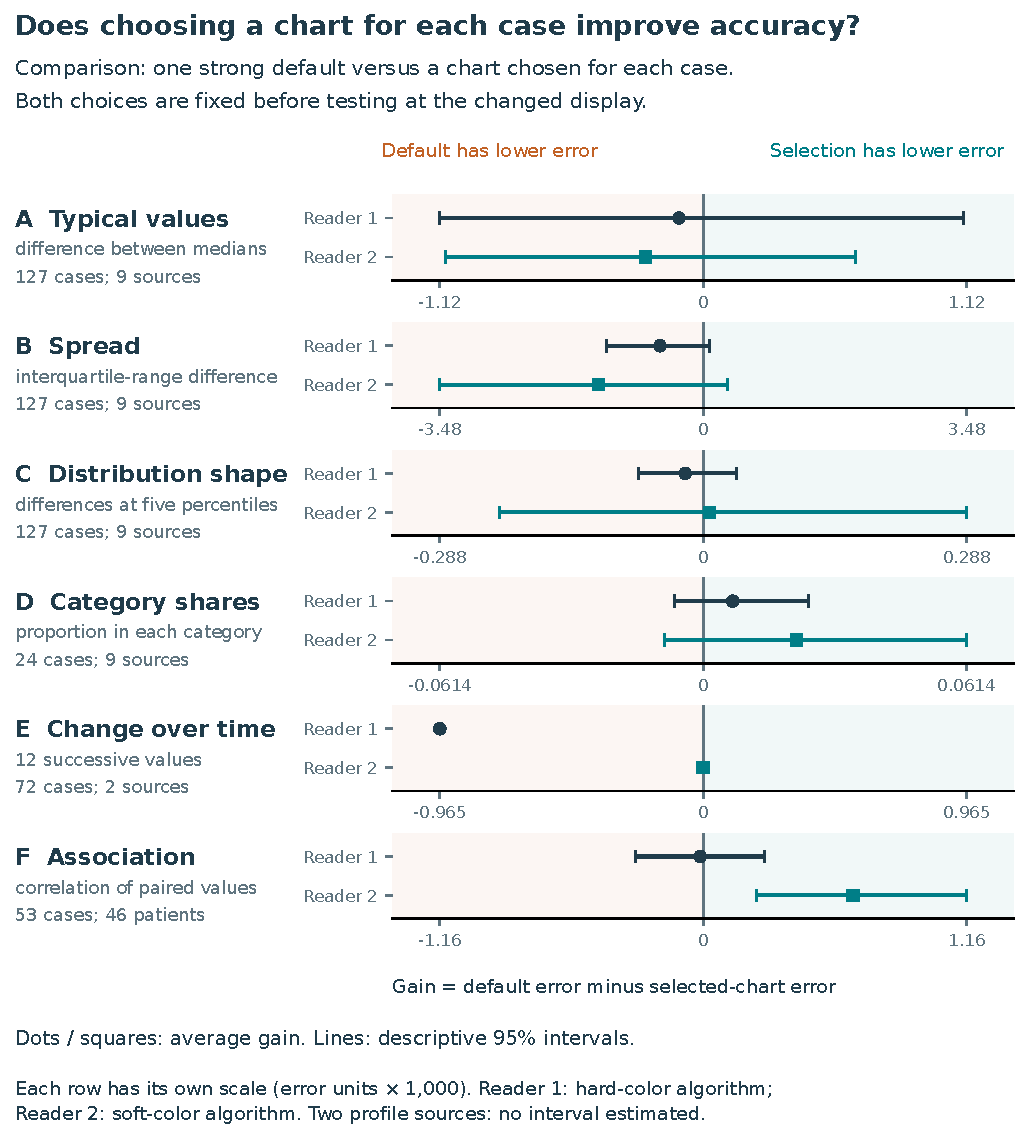
\includegraphics[width=\linewidth]{benchmark_release/figures/Figure_2_Strong_defaults.pdf}
\caption{\textbf{Choosing a chart for each case does not consistently beat a strong default.} Left of zero, the default has lower error; right of zero, case-specific selection has lower error. Points show average paired gains and lines show descriptive 95\% bootstrap intervals. Reader 1 uses hard-color thresholds; Reader 2 uses soft-color weights. These are algorithms, not human participants. Each row has its own numerical scale, enlarged by 1,000 for readability. Resampling uses nine resources for the first four tasks and 46 patients for association; profiles have only two sources and no interval. Repeated recordings are first averaged within participants. Every available Reader 1 interval crosses zero; this does not establish equivalence.}\label{fig:defaults}
\end{figure}

\subsection*{Candidate coverage is part of the result}
Figure~\ref{fig:coverage} makes the familiar candidate set visible. A zero means that a family was tested but never won that task under the specified decoder; a dash means there is no implemented contract. Counts include ties and are conditional on the task and candidate budget. This overview helps readers find the relevant comparison without interpreting an ineligible chart as a poor performer. It does not replace the expanded-control analysis. The original eight-panel display-transfer gallery is retained as Supplementary Figure S1; its deliberately difficult cases illustrate sensitivity rather than its frequency.

\begin{figure}[p]\centering
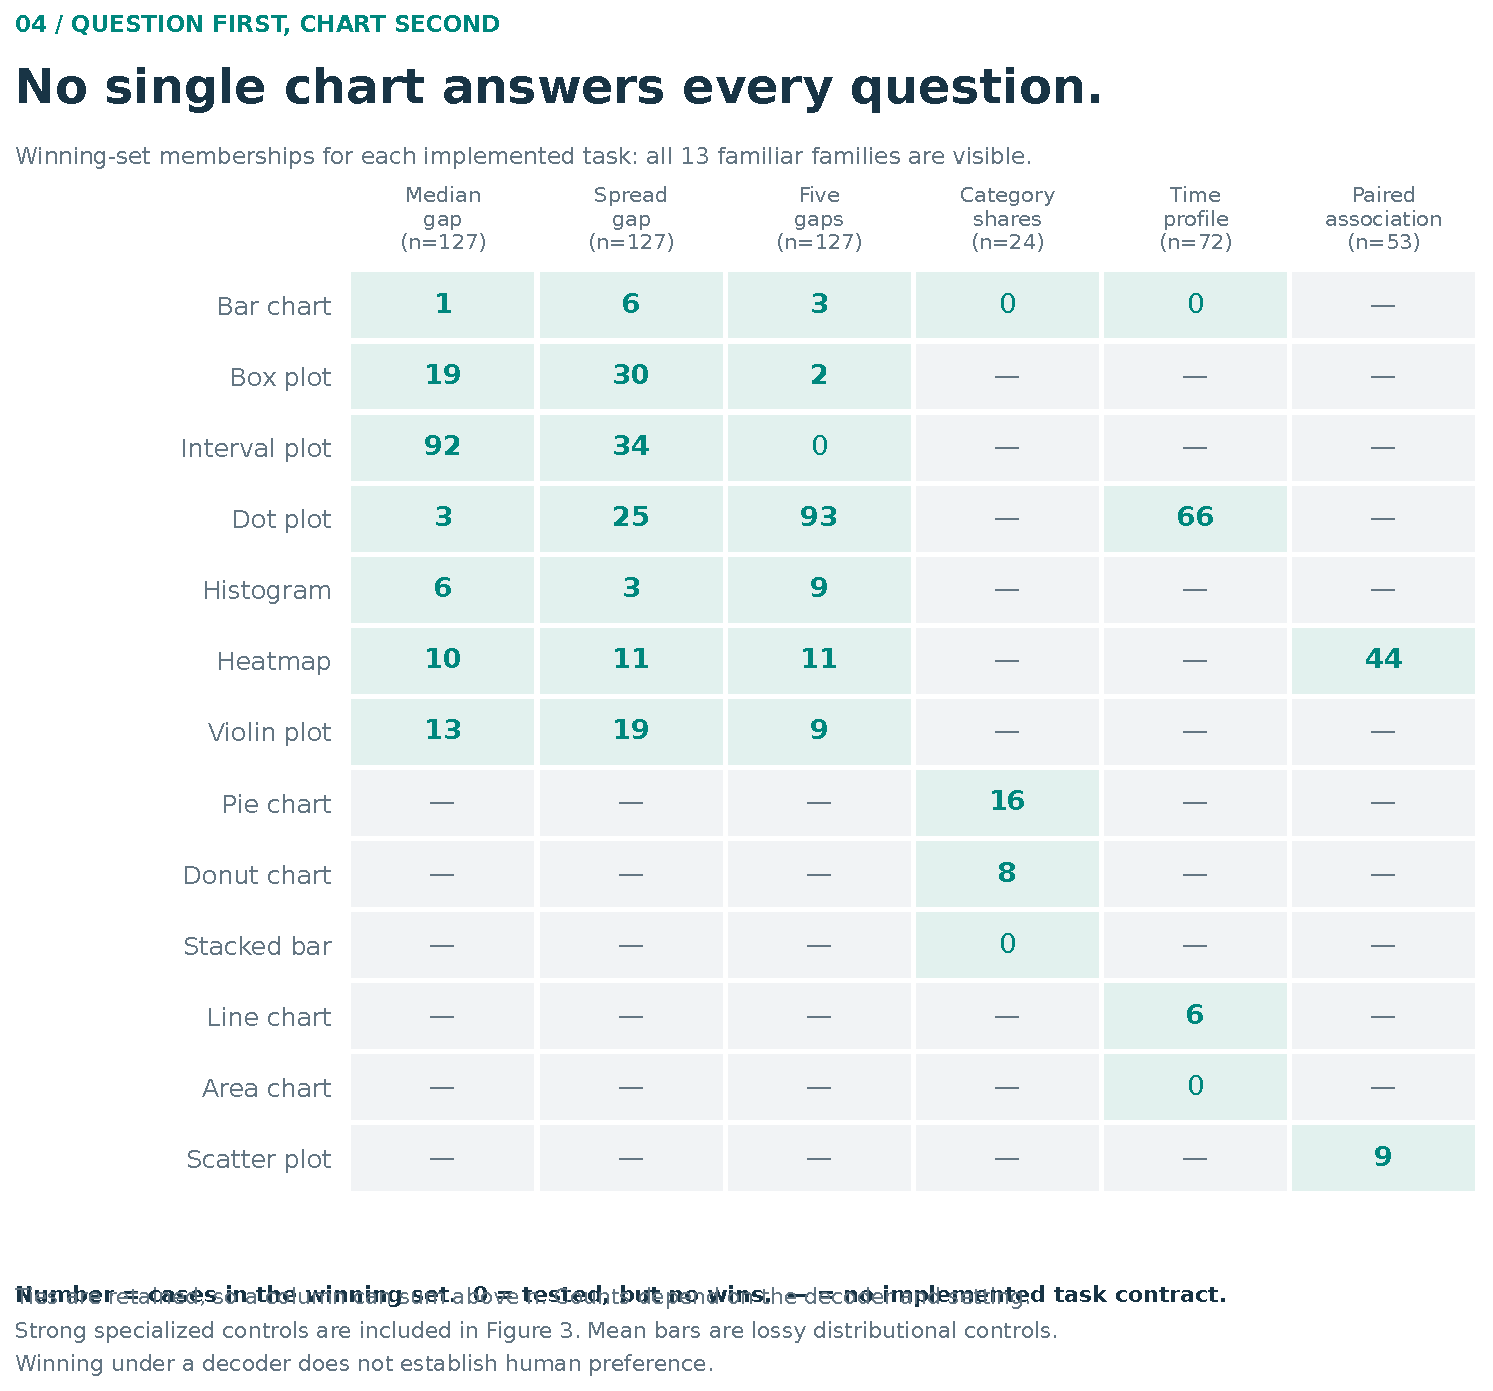
\includegraphics[width=\linewidth,height=.83\textheight,keepaspectratio]{reader_figures/figures/Figure_4_Question_first_chart_second.pdf}
\caption{\textbf{Choose the question before comparing familiar charts.} Reference winning-set memberships for all 13 familiar families under the hard-color algorithm. The marginal columns compare seven fixed familiar implementations; specialized controls are included separately in the primary benchmark. Ties count for every winning member. Zero denotes a tested non-winner; a dash denotes an unimplemented task contract. Mean bars remain explicitly lossy distributional controls. These counts do not measure reader preference or performance.}\label{fig:coverage}
\end{figure}

\subsection*{A separate geometry decoder changes composition rankings}
To test dependence on the recovery mechanism more directly, we implemented a composition decoder that uses angles and lengths instead of total colored area. It samples an angular lattice for pie and donut charts, reads category-bar endpoints and reads stacked-bar segment lengths on a central scanline. It uses the same rendered images and public geometry but no target proportions. This is a separate implementation within the study, not an independent laboratory replication or a human model.

At the reference display, colored-area recovery assigns the winning set to pies in 16 empirical cases and donuts in eight, with no bar wins. Geometry recovery produces \GeometryBar\ bar memberships, \GeometryPie\ pie memberships, \GeometryDonut\ donut memberships and \GeometryStack\ stacked-bar membership (Fig.~\ref{fig:decoder}). Totals exceed 24 because ties are retained. Pies and donuts tie under this angular reader because the sampled ring lies outside the donut hole and their sampled category assignments coincide. Only \GeometryShared\ of 24 cases share a winning family between the two readers.

This experiment demonstrates why a computational ranking must identify its decoder. It does not establish that geometry recovery is preferable. Both readers exploit known chart construction, and neither tests whether a person can quickly or accurately interpret the image. A nearly invisible probability heatmap can likewise retain information for a calibrated machine reader. Color readability and numerical recoverability are distinct properties.\cite{crameri2020}

\begin{figure}[p]\centering
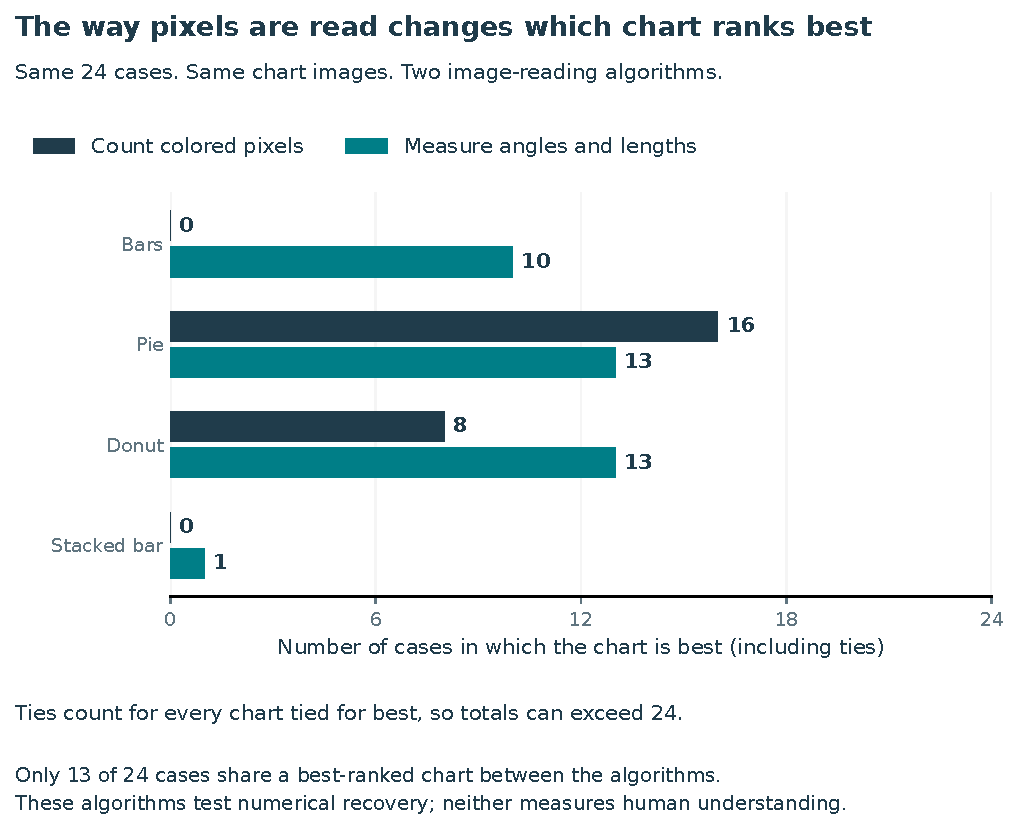
\includegraphics[width=\linewidth]{benchmark_release/figures/Figure_3_Decoder_dependence.pdf}
\caption{\textbf{Changing the image-reading algorithm changes which chart ranks best.} Bars count cases in which each chart has the lowest error among four eligible families. The first algorithm counts colored pixels; the second measures angles and lengths. Both process the same images for all 24 empirical category-share tasks at 256 pixels, averaging four placements. All ties count: pie and donut tie under the angular reader, so the second algorithm's counts total more than 24. Only 13 cases share a best-ranked chart across algorithms. The result concerns numerical recovery, not how well people understand the charts.}\label{fig:decoder}
\end{figure}

\subsection*{New synthetic cases show conditional benefits and losses}
We next froze one default per task and observer using all empirical reference-display results. Newly generated synthetic cases then tested transfer to different inputs as well as the changed display. Thirty-six two-group inputs cover null, location, scale, skew, mixture and heavy-tail regimes at two sample sizes. Forty-eight compositions vary category count and balance. Thirty-six profiles vary shape and amplitude, and 36 paired datasets vary correlation and sample size. Reusing the two-group inputs for three questions produces 228 new task instances from 156 synthetic inputs.

Under the hard decoder, the average gains are $+0.000211$ for composition and $+0.003684$ for association, but $-0.001169$ for median and $-0.002159$ for spread. Five-gap and profile selection tie their frozen defaults in every hard-decoder case. Both observers show positive mean gains for composition and association and negative gains for median and spread. Figure~\ref{fig:synthetic} shows how often selection helps, ties or hurts; Supplementary Figure S2 shows the size of each gain or loss. Counts and mean gains answer different questions: a method can help frequently while producing a large error in a few cases. All selected and default policies decode successfully. Scenario-level results and both observers are retained; no pooled effect across tasks is calculated.

These cases were generated after the new protocol and empirical defaults were fixed. They were not used to tune the defaults. Nevertheless, their design was informed by earlier analyses, and the scenario grid is small. They provide reproducible stress tests, not untouched external-population validation. Their mixed outcomes support conditional usefulness rather than a universal adaptive advantage.

\begin{figure}[p]\centering
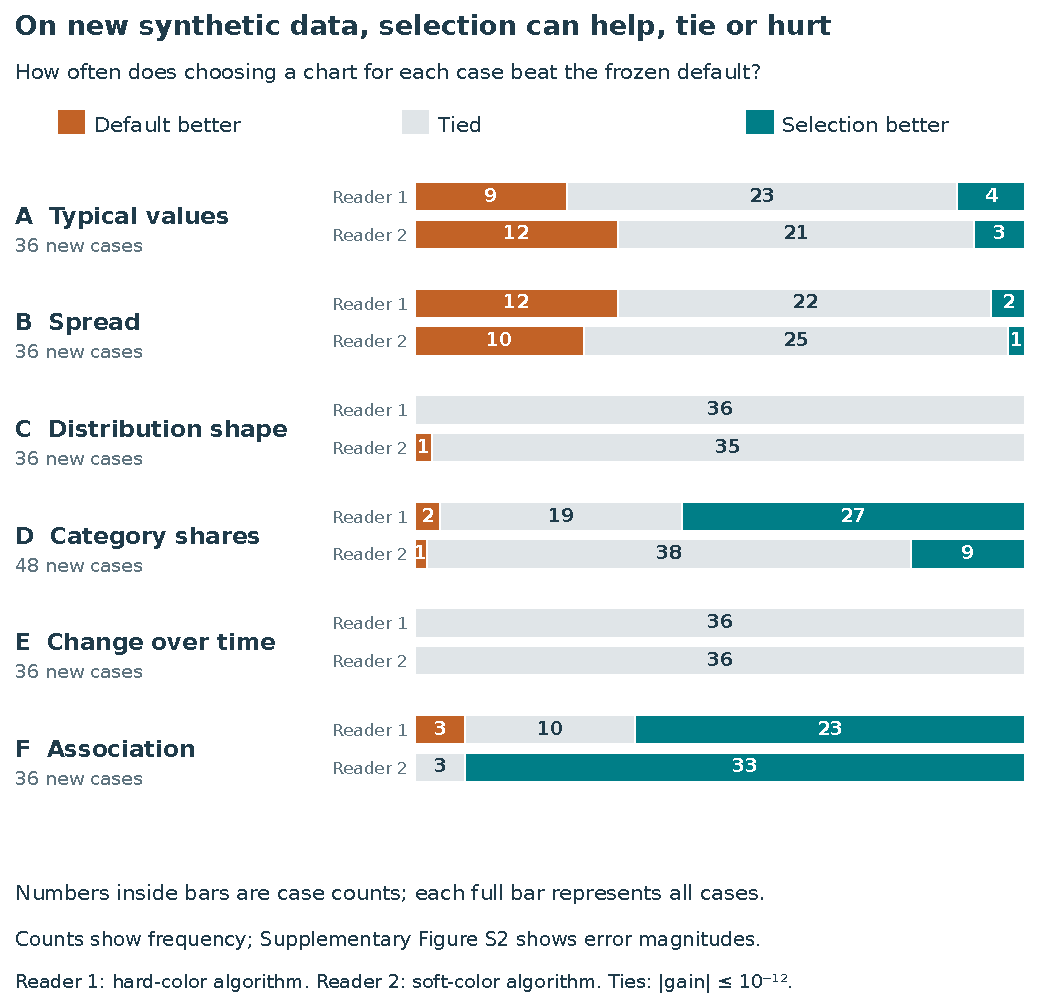
\includegraphics[width=\linewidth]{benchmark_release/figures/Figure_4_Synthetic_transfer.pdf}
\caption{\textbf{Selection helps on some new inputs and hurts on others.} Each bar represents all synthetic cases for one task and algorithm. Segments count cases in which the fixed default has lower error (orange), errors tie (gray), or case-specific selection has lower error (teal). Numbers are counts, not effect sizes; errors within $10^{-12}$ are ties. Reader 1 and Reader 2 are the hard- and soft-color algorithms. Defaults are trained on empirical data. Case-specific choices are made at 256 pixels, frozen, and tested at 384 pixels. Supplementary Figure S2 retains individual gains and their means. The designed scenarios are stress tests, not a sample of a population.}\label{fig:synthetic}
\end{figure}

\subsection*{Information loss, recovery error and transfer are separate}
Three tests explain what a score can establish. First, a chart must carry the requested information. Two datasets can have the same group means and variances but different quantile differences; identical mean-only charts cannot distinguish them. Likewise, re-pairing observations preserves marginal distributions but can change the median within-person change. Such a paired target requires pairing information and is rejected for marginal-only charts.

Second, a representation that contains the target can still lose accuracy when rendered or decoded. Explicit quantile markers provide a useful control because they encode the requested values directly. Their errors isolate finite-display and recovery behavior more closely than a comparison with mean bars. Supplementary analyses also separate group-level recovery from contrast recovery: errors shared by the two groups can cancel, yielding a high difference score despite inaccurate group estimates.

Third, a reference-display winner may not remain best after the display changes. An elementary bound clarifies this. If all candidates are valid in both conditions and each loss changes by at most $\epsilon$, then the frozen winner's excess test loss is at most $2\epsilon+\tau$, where $\tau=10^{-12}$ is the selection tolerance. The proof and case-level checks appear in the Supplement. This bound explains why rank stability depends on the size of environmental perturbations; it is not a new optimization theorem or a guarantee about untested displays.

\section*{Discussion}
The benchmark turns a broad chart-choice question into a testable sequence: specify the answer, recover it from pixels, and compare the selected chart with a strong default under changed conditions. Its contribution is the executable evaluation and the evidence it exposes. Numerical optimization on the reference display works by construction. Added value after transfer must be demonstrated separately.

This distinction matters for scientists, visualization developers and teachers. A researcher can use a task specification to identify information that a proposed chart omits. A developer can test a renderer or decoder without calling its score a measure of comprehension. A teacher can contrast the difference between an adequate encoding, an accurate machine readout and a useful human-facing display. A researcher interested in communication still needs evidence about readers. Distribution-preserving alternatives to mean-only summaries remain important, but that principle does not establish which implementation is best in every setting.\cite{weissgerber2015,rousselet2017}

For practical use, the workflow has three steps. First, state the numerical question and select a compatible input format. Second, render the eligible candidates and compare the frozen choice with a task-matched default at the intended display conditions. Third, inspect the absolute errors, failures and decoder sensitivity alongside the chart. If the result depends on the decoder or offers negligible improvement, the numerical ranking alone supplies no reason to replace a familiar, appropriate default. This is an interpretation rule, not a validated human-performance threshold. The supplied CSV interface produces the inputs, all scores and a default-versus-selection summary so this comparison can be checked on another dataset.

Strong defaults are an essential part of this evaluation. A five-marker distributional control may be less familiar than a box plot, but excluding it would weaken a claim about preserving five requested quantiles. We retain familiar charts for accessibility and explicit controls for a fair test. Likewise, the synthetic association benefit is informative precisely because the empirical association result depends on the observer. Both outcomes belong in the evidence base.

Several limits define the scope. The benchmark is retrospective, and its public resources are a convenience sample. Multiple features share cohorts and several recordings share patients. Source and patient grouping reduce obvious dependence but cannot make nine resources representative of science. The profile comparison uses only two sources, and the association comparison comes from one source. Dataset-specific ambiguities are retained and documented rather than silently corrected. Sensitivity analyses accompany the original arrays.

The decoder is another substantive limitation. The two original observers share known axes and much geometry. The new composition reader uses a different extraction mechanism but still assumes known construction. Color, blur, overlap, line thickness, axis padding and tuning budgets can affect rankings. The transfer changes both resolution and placement; it does not isolate a causal effect of resolution alone. Accessibility, semantics, reading time, visual salience and scientific usefulness are not evaluated. No aggregate score combines these unmeasured dimensions.

The package makes future disagreement testable: another investigator can replace the renderer, decoder, task or candidate set and compare against the same fixed defaults. The accompanying prospective protocol specifies how to evaluate frozen predictions against human estimation error, time and confidence on new examples. No reader recruitment or reader outcomes are claimed here. Until such evidence exists, the appropriate interpretation is a computational benchmark of recoverable information.

\section*{Methods}
\subsection*{Data and task construction}
The two-group benchmark comprises WDBC (30 features), Cleveland (5), heart failure (6), CKD (11), ILPD (9), retinopathy (16), HAR (40), BIDMC (5) and wrist exercise (5).\cite{wdbc,heart,failure,kidney,liver,retina,har,bidmc,wrist} HAR uses subject/activity medians. BIDMC aggregates source readings within 46 patients; wrist uses early/late summaries within eight participants.\cite{pimentel2017,jarchi2017} Parkinsons is excluded from the primary comparisons because parsed identifiers do not reconcile with the documented participant count. Retinopathy linkage and two CKD potassium values remain unresolved; omission sensitivities are preserved in the release.

For each resource, pooled quartiles of the first canonical feature define four composition categories for each group, yielding 18 cases. Six unpaired resources contribute observed binary group shares, giving 24 compositions. These are proportions among included records, not disease prevalence. Profiles use 12 equal-duration bin means from 19 wrist and 53 BIDMC recordings. Associations use positive valid paired ECG-HR and pulse readings from each BIDMC recording, systematically subsampled to at most 64 rows. Pearson correlation targets the displayed subset and does not measure agreement.

For marginal tasks, $d_p=Q_y(p)-Q_x(p)$ uses linear empirical quantiles. Targets are $d_{.5}$, $d_{.75}-d_{.25}$ and $(d_{.1},d_{.25},d_{.5},d_{.75},d_{.9})$. Absolute errors are divided by pooled within-group SD. The constant-scale fallback and its loss of unit invariance are documented in the Supplement. Composition loss is half the summed absolute share error. Profile loss is mean absolute error divided by the SD of the twelve true bin means. Association loss is half the absolute correlation error. Small profile SD can amplify small absolute errors; absolute targets and recovered values are retained for inspection.

\subsection*{Rendering and recovery}
Each marginal task compares seven familiar fixed configurations, an ECDF and five- and nineteen-quantile marker controls. Composition uses bars, pies, donuts and stacked bars; profiles use lines, areas, dots and bars; association uses scatter plots and probability heatmaps. Geometries, colors, bin counts and stroke widths are fixed. Rendering uses fourfold supersampling, Lanczos reduction and 0.5-pixel Gaussian blur. Reference panels use 256 pixels and placements $0,.25,.5,.75$; test panels use 384 pixels and placements $.125,.375,.625,.875$.

The hard observer uses color-distance thresholds; the soft observer uses color-projection weights, with task-specific geometry rules. Marginal readers recover quantiles from landmarks or cumulative pixel mass. Profile readers use mark centroids or upper boundaries. Association readers recover correlation from scatter pixel mass or probability-cell mass. The separate geometry reader applies 4,096 angular samples at 76\% of the nominal radius, bar endpoints and stacked-bar scanline lengths. It receives no subpixel phase. Full contracts and failure rules are provided in the Supplement and source code.

\subsection*{Default selection, dependence and uncertainty}
One fixed default is learned per task and observer by excluding the held-out resource and minimizing resource-balanced reference loss. Recording-level losses first average within participants for profiles. For association, the held-out patient's recordings are excluded together and training patients receive equal weight. A candidate with any failed training placement is ineligible as a learned default. Case-specific selection renders every eligible candidate and uses that case's reference losses, calculated against the known source-data target. Source observations are withheld from the decoder, not from the evaluator. The method is therefore an exhaustive computational audit, not a recommender that predicts a chart without evaluating alternatives. All losses within $10^{-12}$ of the minimum are scientific ties; a fixed candidate order selects a representative for deployment.

At the test display, policies are compared on paired valid cases and failures are reported separately. Default and selected losses are averaged within resource after participant aggregation where appropriate. Association weights patients equally. Descriptive percentile intervals use 5,000 paired resamples of nine resource means or 46 patient means. Only two profile resources are available, so no interval is estimated. Intervals are neither multiplicity-adjusted confirmatory tests nor estimates for a random sample of all scientific datasets.

\subsection*{Synthetic design and verification}
The new protocol was written before the revision analyses, after the earlier results had been inspected. Seed 2026092201 generates the synthetic inputs. Two-group cases cross six regimes with $n=30,150$ and three replicates. Compositions cross 2, 3, 5 or 8 categories with Dirichlet concentrations 0.3, 1 or 5 and four replicates. Profiles cross ramp, wave or step shapes with relative amplitudes 0.01, 0.1 or 0.4 and four replicates. Associations cross correlations $-0.8,0,0.8$ with 16, 64 or 256 displayed pairs and four replicates. Their targets are empirical quantities in each generated input, not theoretical population parameters.

Verification reruns the empirical render--decode analyses, compares configuration losses with the supplied release, recomputes new synthetic losses from saved recovered values and source arrays, checks held-out-unit exclusion, and checks that policy losses come from the test display. Blank images must fail. Unit-scaling and metadata tests accompany the original decoders and control implementations. Machine-readable inputs, raw sources, recovered values, failures, fold assignments, software versions and checksums are included. Tests establish computational consistency within this environment, not external replication or human validity.

\section*{Data availability}
The cited UCI and PhysioNet resources provide the original data. The accompanying reproducibility package contains the source copies used here, prepared arrays, task transformations, new synthetic inputs and case-level results, subject to the original terms and attribution recorded in \texttt{DATA\_PROVENANCE.md}. Synthetic observations are explicitly labeled. No new participant or human-reader data were collected.

\section*{Code availability}
The accompanying version 5.0 reproducibility package contains code, input data and pinned dependency specifications. After installing the dependencies, the primary results can be rebuilt offline. \texttt{python reproduce\_benchmark.py --full} rebuilds inputs, empirical and synthetic evaluations, comparisons, checks, tables and figures; \texttt{--verify} audits saved results. \texttt{score\_task.py} supplies task-specific CSV examples, and \texttt{benchmark\_release/score\_and\_compare.py} adds expanded marginal controls and frozen-default comparisons. Project repository: \url{https://github.com/Elgendi/two-sample-chart-selection}. The accompanying versioned package is the computational record; the repository must be synchronized with this release before it can serve as the reproduction source.

\section*{Author contributions}
M.E. conceived the study, developed the methodological approach, interpreted the analyses and prepared the manuscript. The computational implementation and manuscript revision used AI assistance; the author is responsible for verification and final approval.
\section*{Competing interests}
M.E. serves on the editorial boards of Communications Medicine and npj Biosensing. The author declares no other competing interests.
% AUTHOR ACTION: insert the verified funding statement and corresponding-author email before submission; neither was supplied in the source manuscript.
\begingroup\small\setlength{\bibsep}{2pt}\bibliographystyle{viznumbered}\bibliography{references}\endgroup
\end{document}
